\documentclass[11pt]{article}
\usepackage[margin=1in]{geometry}
\usepackage{xcolor}
\usepackage{mdframed}
\usepackage{amsmath}
\usepackage{graphicx}
\usepackage{float}
\usepackage{listings}
\usepackage{hyperref}

\lstset{
    language=Matlab,
    basicstyle=\ttfamily\footnotesize,
    keywordstyle=\color{blue},
    breaklines=true
}

\newcommand{\yourname}{Alex Shaffer, Istiaque Ahmed}
\newcommand{\yournetid}{aws9, miahmed2}
\newcommand{\hwnum}{4}
\newcommand{\probnum}{1}

\newenvironment{problem}[2][Problem]
    { \begin{mdframed}[backgroundcolor=gray!20] \textbf{#1 #2} \\}
    {  \end{mdframed}}

\newenvironment{solution}
    {\textit{Solution:}}
    {}

\begin{document}
\noindent
\noindent\rule{\linewidth}{2pt}
\large\textbf{\yourname} \hfill \textbf{CS 555: Homework \# \hwnum}   \\
Email: \yournetid@illinois.edu \hfill Spring 2026\\
GitHub Repo: \texttt{\url{https://github.com/redhorn144/CS555/}} \\
\noindent\rule{\linewidth}{2pt}

% -------------------------------------------------------
\begin{problem}{1(a)}
Solve the steady-state advection-diffusion problem on $\Omega=[0,1]$ with uniform elements ($E=100$),
$u(0)=u(1)=0$, $\nu=10^{-3}$, $f=1$. Report the maximum pointwise relative error.
\end{problem}

\begin{solution}

Consider the steady-state advection-diffusion problem on $\Omega = [0,1]$:
\begin{equation}
    c u_x = \nu u_{xx} + f
\end{equation}
with boundary conditions $u(0) = u(1) = 0$. The parameters are $L=1$, $c=1$, $\nu=10^{-3}$, and $f=1$.

\subsection*{Analytical Solution}
The exact analytical solution is required to compute the pointwise relative error. The general solution is:
\begin{equation}
    u(x) = C_1 + C_2 e^{\frac{c}{\nu}x} + \frac{f}{c}x
\end{equation}
Applying the Dirichlet boundary conditions yields:
\begin{equation}
    u(x) = \frac{f}{c} \left( x - \frac{e^{\frac{c}{\nu}x} - 1}{e^{\frac{c}{\nu}L} - 1} \right)
\end{equation}
To avoid floating-point overflow during computation ($\frac{c}{\nu} = 1000$), the exact solution is approximated by the stable boundary layer form:
\begin{equation}
    u(x) \approx x - e^{\frac{c}{\nu}(x - 1)}
\end{equation}

\subsection*{Finite Element Formulation}
The domain is discretized into $E=100$ uniform elements with $h_e = 0.01$. Linear basis functions are utilized. The element matrices are:
\begin{equation}
    A^e = \frac{1}{h_e} \begin{bmatrix} 1 & -1 \\ -1 & 1 \end{bmatrix}, \quad
    C^e = \frac{1}{2} \begin{bmatrix} -1 & 1 \\ -1 & 1 \end{bmatrix}, \quad
    F^e = \frac{f h_e}{2} \begin{bmatrix} 1 \\ 1 \end{bmatrix}
\end{equation}
The global system $( \nu A + c C ) \underline{u} = F$ is assembled and solved after applying the boundary conditions.

\subsection*{Results}
The local element P\'eclet number is $Pe = \frac{c h_e}{2\nu} = 5$. Because $Pe > 1$, the standard Galerkin formulation exhibits severe non-physical spatial oscillations near the right boundary ($x=1$).

The computed maximum pointwise relative error is \textbf{0.6735}.

\begin{figure}[H]
    \centering
    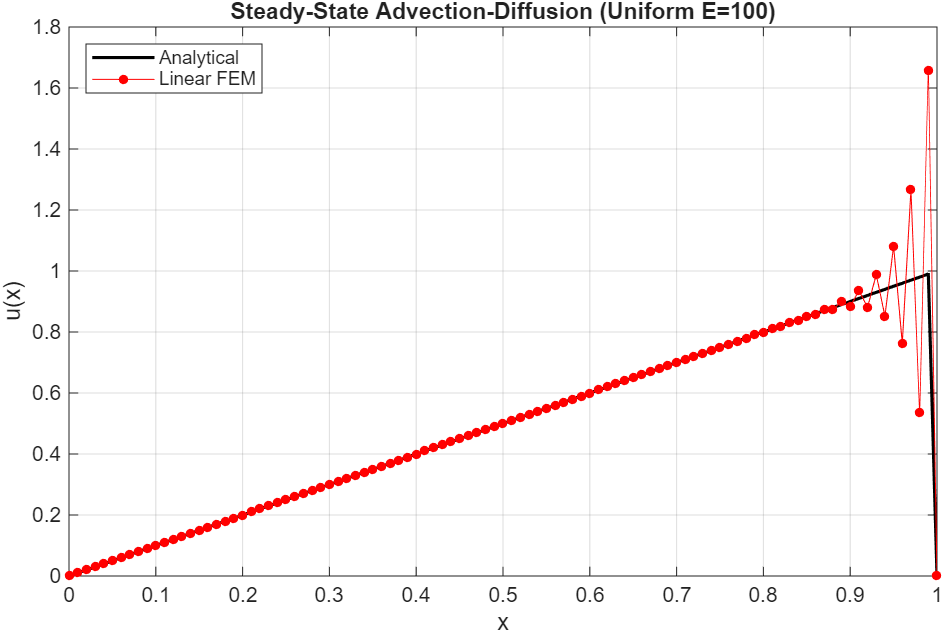
\includegraphics[width=0.7\textwidth]{1_a.png}
    \caption{Steady-State Advection-Diffusion using a uniform mesh ($E=100$).}
    \label{fig:1a}
\end{figure}

\subsection*{MATLAB Implementation}
\begin{lstlisting}
L = 1.0; c = 1.0; nu = 1e-3; f = 1.0;
E = 100; N = E + 1; h = L / E;

x = linspace(0, L, N)';
K = sparse(N, N);
F = zeros(N, 1);

for e = 1:E
    A_e = (1.0 / h) * [1.0, -1.0; -1.0, 1.0];
    C_e = 0.5 * [-1.0, 1.0; -1.0, 1.0];
    idx = [e, e+1];
    K(idx, idx) = K(idx, idx) + nu * A_e + c * C_e;
    F(idx) = F(idx) + (f * h / 2.0) * [1.0; 1.0];
end

K(1, :) = 0.0; K(1, 1) = 1.0; F(1) = 0.0;
K(end, :) = 0.0; K(end, end) = 1.0; F(end) = 0.0;

u_h = K \ F;

u_ex = x - exp((c / nu) * (x - L));
u_ex(1) = 0.0; u_ex(end) = 0.0;

interior_idx = 2:(N-1);
rel_error = max(abs(u_ex(interior_idx) - u_h(interior_idx)) ./ abs(u_ex(interior_idx)));
fprintf('Maximum pointwise relative error: %.4e\n', rel_error);
\end{lstlisting}

\end{solution}

% -------------------------------------------------------
\begin{problem}{1(b)}
Repeat 1(a) with nonuniform elements ($E=20$) using a geometric progression $L_e = s L_{e-1}$ with $s=0.7$.
Report the maximum pointwise relative error.
\end{problem}

\begin{solution}

The steady-state advection-diffusion problem is solved using a nonuniform mesh with $E=20$ elements. The element lengths follow a geometric progression $L_e = s L_{e-1}$ with a scale factor of $s=0.7$. The length of the first element is determined by the geometric series sum:
\begin{equation}
    L_1 = L \frac{1 - s}{1 - s^E}
\end{equation}

\subsection*{Results}
By geometrically clustering the elements near the right boundary ($x=1$), the local element P\'eclet number in the steep boundary layer region is significantly reduced. This mitigates the spatial oscillations observed in the uniform mesh approach. The computed maximum pointwise relative error is \textbf{0.0120} ($1.1972 \times 10^{-2}$).

\begin{figure}[H]
    \centering
    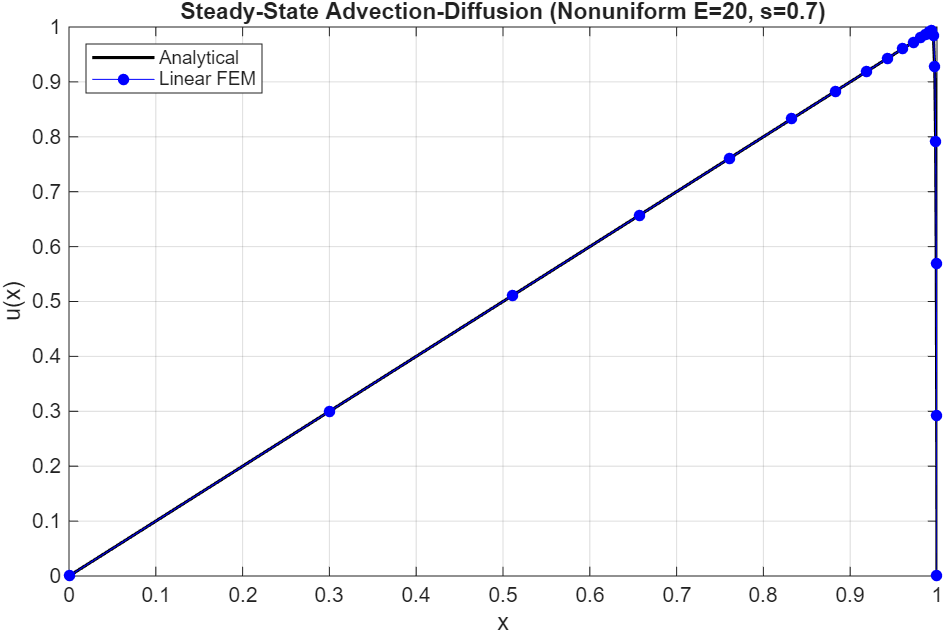
\includegraphics[width=0.7\textwidth]{1_b.png}
    \caption{Steady-State Advection-Diffusion using a nonuniform mesh ($E=20, s=0.7$).}
    \label{fig:1b}
\end{figure}

\subsection*{MATLAB Implementation}
\begin{lstlisting}
L = 1.0; c = 1.0; nu = 1e-3; f = 1.0;
E = 20; N = E + 1; s = 0.7;

L1 = L * (1 - s) / (1 - s^E);
Le = L1 * s.^(0:E-1);
x = [0, cumsum(Le)]';

K = sparse(N, N);
F = zeros(N, 1);

for e = 1:E
    h_e = Le(e);
    A_e = (1.0 / h_e) * [1.0, -1.0; -1.0, 1.0];
    C_e = 0.5 * [-1.0, 1.0; -1.0, 1.0];
    idx = [e, e+1];
    K(idx, idx) = K(idx, idx) + nu * A_e + c * C_e;
    F(idx) = F(idx) + (f * h_e / 2.0) * [1.0; 1.0];
end

K(1, :) = 0.0; K(1, 1) = 1.0; F(1) = 0.0;
K(end, :) = 0.0; K(end, end) = 1.0; F(end) = 0.0;

u_h = K \ F;

u_ex = x - exp((c / nu) * (x - L));
u_ex(1) = 0.0; u_ex(end) = 0.0;

interior_idx = 2:(N-1);
rel_error = max(abs(u_ex(interior_idx) - u_h(interior_idx)) ./ abs(u_ex(interior_idx)));
fprintf('Maximum pointwise relative error: %.4e\n', rel_error);
\end{lstlisting}

\end{solution}

% -------------------------------------------------------
\begin{problem}{1(c)}
For $E=20$, find a value of $s$ that minimizes the pointwise error by trial and error.
\end{problem}

\begin{solution}

To find the scale factor $s$ that minimizes the pointwise error for the nonuniform mesh with $E=20$ elements, a parameter sweep is performed for $s \in [0.5, 0.95]$. For each value of $s$, the mesh is generated, the finite element system is assembled and solved, and the maximum pointwise relative error is computed.

\subsection*{Results}
The parameter sweep reveals a distinct minimum in the error curve. The optimal scale factor is found to be \textbf{0.65}, which yields a minimum maximum pointwise relative error of \textbf{0.0088} ($8.8193 \times 10^{-3}$). This value optimally balances the resolution within the steep boundary layer against the resolution in the remainder of the domain.

\begin{figure}[H]
    \centering
    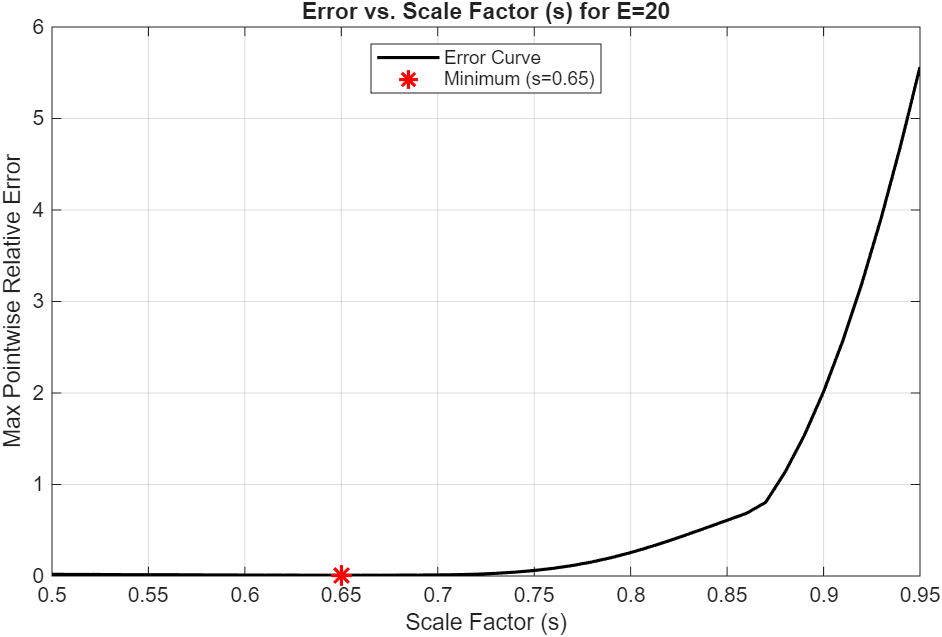
\includegraphics[width=0.7\textwidth]{1_c.png}
    \caption{Error vs. Scale Factor (s) for $E=20$, showing the minimum at $s=0.65$.}
    \label{fig:1c}
\end{figure}

\subsection*{MATLAB Implementation}
\begin{lstlisting}
L = 1.0; c = 1.0; nu = 1e-3; f = 1.0;
E = 20; N = E + 1;

s_vals = 0.5:0.01:0.95;
errors = zeros(length(s_vals), 1);

for k = 1:length(s_vals)
    s = s_vals(k);

    L1 = L * (1 - s) / (1 - s^E);
    Le = L1 * s.^(0:E-1);
    x = [0, cumsum(Le)]';

    K = sparse(N, N);
    F = zeros(N, 1);

    for e = 1:E
        h_e = Le(e);
        A_e = (1.0 / h_e) * [1.0, -1.0; -1.0, 1.0];
        C_e = 0.5 * [-1.0, 1.0; -1.0, 1.0];
        idx = [e, e+1];
        K(idx, idx) = K(idx, idx) + nu * A_e + c * C_e;
        F(idx) = F(idx) + (f * h_e / 2.0) * [1.0; 1.0];
    end

    K(1, :) = 0.0; K(1, 1) = 1.0; F(1) = 0.0;
    K(end, :) = 0.0; K(end, end) = 1.0; F(end) = 0.0;

    u_h = K \ F;

    u_ex = x - exp((c / nu) * (x - L));
    u_ex(1) = 0.0; u_ex(end) = 0.0;

    interior_idx = 2:(N-1);
    rel_error = abs(u_ex(interior_idx) - u_h(interior_idx)) ./ abs(u_ex(interior_idx));
    errors(k) = max(rel_error);
end

[min_err, min_idx] = min(errors);
opt_s = s_vals(min_idx);

fprintf('Optimal s value: %.2f\n', opt_s);
fprintf('Minimum maximum pointwise relative error: %.4e\n', min_err);
\end{lstlisting}

\end{solution}

% -------------------------------------------------------
\begin{problem}{2(a)}
Solve the unsteady advection-diffusion problem with $f=0$, $u^0=0$, $u(0,t)=\sin(\pi t)$, $u(1,t)=0$
using BDF3/EXT3 and $E=100$ uniform elements. Plot the solution at $t=1.5$ and discuss observed errors.
\end{problem}

\begin{solution}

The unsteady advection-diffusion problem is solved using linear finite elements in space ($E=100$, uniform) and a 3rd-order Backward Differentiation Formula with 3rd-order explicit extrapolation (BDF3/EXT3) in time. The diffusion term is treated implicitly, while the advection term is treated explicitly to avoid solving a non-symmetric system.

\subsection*{Time Integration Scheme}
The semi-discrete system is:
\begin{equation}
    B\underline{u}_t + cC\underline{u} = -\nu A\underline{u}
\end{equation}
The BDF3/EXT3 scheme requires bootstrapping the first two time steps. Let $\Delta t = 0.001$.
\begin{itemize}
    \item \textbf{Step 1 (BDF1/EXT1):} $\left(\frac{1}{\Delta t} B + \nu A\right) u^1 = \frac{1}{\Delta t} B u^0 - c C u^0$
    \item \textbf{Step 2 (BDF2/EXT2):} $\left(\frac{3}{2\Delta t} B + \nu A\right) u^2 = \frac{1}{\Delta t} B \left(2 u^1 - \frac{1}{2} u^0\right) - c C (2 u^1 - u^0)$
    \item \textbf{Step 3+ (BDF3/EXT3):}
    \begin{equation*}
        \left(\frac{11}{6\Delta t} B + \nu A\right) u^{n+1} = \frac{1}{\Delta t} B \left(3 u^n - \frac{3}{2} u^{n-1} + \frac{1}{3} u^{n-2}\right) - c C \left(3 u^n - 3 u^{n-1} + u^{n-2}\right)
    \end{equation*}
\end{itemize}

\subsection*{Results and Error Analysis}
The solution at $t=1.5$ is subjected to the Dirichlet boundary conditions $u(0,t) = \sin(\pi t)$ and $u(1,t) = 0$.

Observing the wave profile, the primary numerical artifact is the presence of \textbf{trailing oscillations} behind the main wave. This is a symptom of \textbf{numerical dispersion} (phase error). Because standard Galerkin linear finite elements lack stabilization (such as upwinding), the higher-frequency components of the numerical solution travel at slower wave speeds than the exact physical speed, causing them to lag and form a dispersive tail.

The right boundary condition being Dirichlet is non-physical because the wave is meant to outflow freely. The enforced zero value at $x=1$ creates a sharp gradient as the wave approaches the boundary, which exacerbates the dispersive oscillations.

\begin{figure}[H]
    \centering
    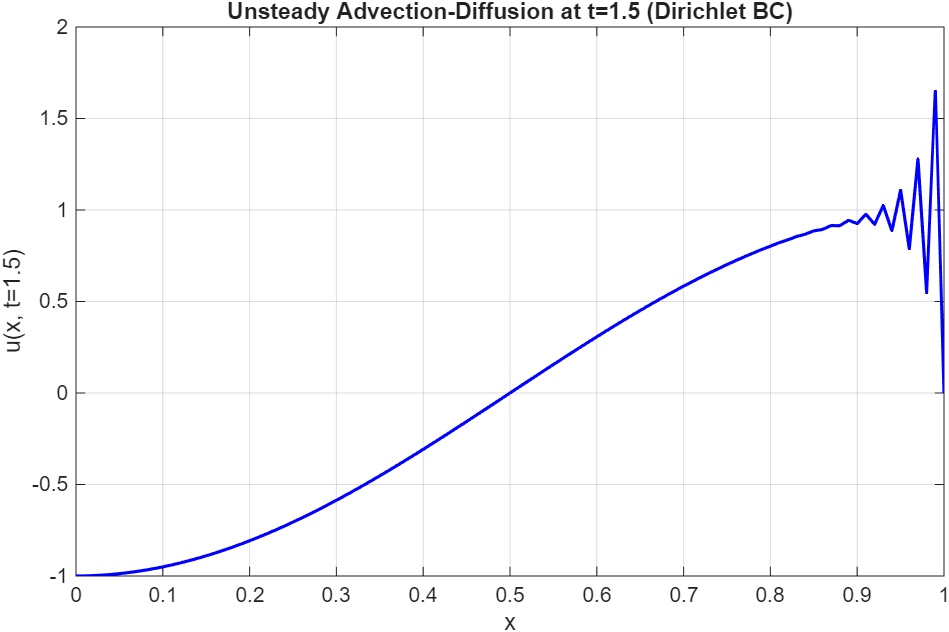
\includegraphics[width=0.7\textwidth]{2_a.png}
    \caption{Unsteady Advection-Diffusion at $t=1.5$ with Dirichlet BCs.}
    \label{fig:2a}
\end{figure}

\subsection*{MATLAB Implementation}
\begin{lstlisting}
L = 1.0; c = 1.0; nu = 1e-3; f = 0.0;
E = 100; N = E + 1; h = L / E;
dt = 0.001; t_end = 1.5;
n_steps = round(t_end / dt);

x = linspace(0, L, N)';
A = sparse(N, N); C = sparse(N, N); B = sparse(N, N);

for e = 1:E
    A_e = (1.0 / h) * [1.0, -1.0; -1.0, 1.0];
    C_e = 0.5 * [-1.0, 1.0; -1.0, 1.0];
    B_e = (h / 6.0) * [2.0, 1.0; 1.0, 2.0];

    idx = [e, e+1];
    A(idx, idx) = A(idx, idx) + A_e;
    C(idx, idx) = C(idx, idx) + C_e;
    B(idx, idx) = B(idx, idx) + B_e;
end

U = zeros(N, n_steps + 1);

LHS1 = (1/dt)*B + nu*A;
LHS2 = (3/(2*dt))*B + nu*A;
LHS3 = (11/(6*dt))*B + nu*A;

for n = 1:n_steps
    t_next = n * dt;

    if n == 1
        RHS = (1/dt)*B*U(:, n) - c*C*U(:, n);
        LHS = LHS1;
    elseif n == 2
        RHS = (1/dt)*B*(2*U(:, n) - 0.5*U(:, n-1)) - c*C*(2*U(:, n) - U(:, n-1));
        LHS = LHS2;
    else
        RHS = (1/dt)*B*(3*U(:, n) - 1.5*U(:, n-1) + (1/3)*U(:, n-2)) - ...
              c*C*(3*U(:, n) - 3*U(:, n-1) + U(:, n-2));
        LHS = LHS3;
    end

    LHS_bc = LHS;
    LHS_bc(1, :) = 0; LHS_bc(1, 1) = 1; RHS(1) = sin(pi * t_next);
    LHS_bc(end, :) = 0; LHS_bc(end, end) = 1; RHS(end) = 0;

    U(:, n+1) = LHS_bc \ RHS;
end
\end{lstlisting}

\end{solution}

% -------------------------------------------------------
\begin{problem}{2(b)}
Repeat 2(a) but change the right boundary condition to $\frac{\partial u}{\partial x}\big|_{x=L} = 0$.
Plot the solution at $t=1.5$ and discuss differences from 2(a).
\end{problem}

\begin{solution}

The right boundary condition is changed from a Dirichlet condition ($u(1,t)=0$) to a homogeneous Neumann condition ($\frac{\partial u}{\partial x}\big|_{x=L}=0$).

\subsection*{Finite Element Implementation}
In the finite element method, Dirichlet conditions are essential boundary conditions that must be explicitly enforced by modifying the global algebraic system (clamping the matrix row). Conversely, Neumann conditions are natural boundary conditions. Because the prescribed flux is zero, the boundary term in the weak formulation naturally vanishes. Therefore, to implement this condition, the explicit clamping of the last row of the global matrix and load vector is simply removed.

\subsection*{Results and Comparison}
Comparing the solution at $t=1.5$ to the results from part 2(a), the differences can be seen at the right boundary ($x=1$).

In 2(a), the Dirichlet condition forced the solution to zero creating a sharp, unnatural gradient as the wave propagated to the right in the domain. In 2(b), the natural Neumann condition allows the wave to advect freely out of the domain. The value at $x=1$ is non-zero, and the spatial derivative (slope) flattens to exactly zero at the boundary, satisfying the homogeneous condition.

\begin{figure}[H]
    \centering
    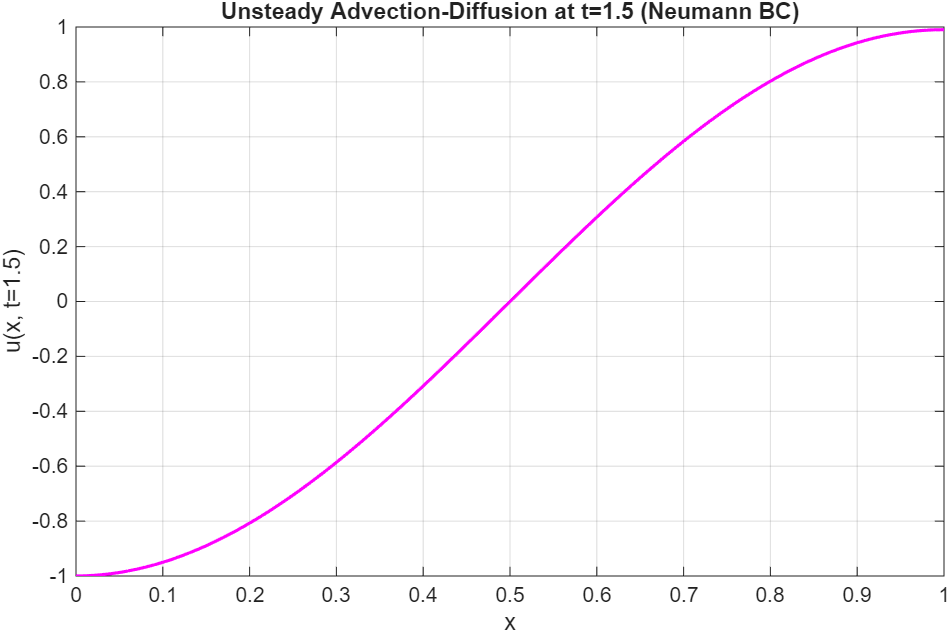
\includegraphics[width=0.7\textwidth]{2_b.png}
    \caption{Unsteady Advection-Diffusion at $t=1.5$ with a Neumann right boundary condition.}
    \label{fig:2b}
\end{figure}

\subsection*{MATLAB Implementation}
\begin{lstlisting}
L = 1.0; c = 1.0; nu = 1e-3; f = 0.0;
E = 100; N = E + 1; h = L / E;
dt = 0.001; t_end = 1.5;
n_steps = round(t_end / dt);

x = linspace(0, L, N)';
A = sparse(N, N); C = sparse(N, N); B = sparse(N, N);

for e = 1:E
    A_e = (1.0 / h) * [1.0, -1.0; -1.0, 1.0];
    C_e = 0.5 * [-1.0, 1.0; -1.0, 1.0];
    B_e = (h / 6.0) * [2.0, 1.0; 1.0, 2.0];

    idx = [e, e+1];
    A(idx, idx) = A(idx, idx) + A_e;
    C(idx, idx) = C(idx, idx) + C_e;
    B(idx, idx) = B(idx, idx) + B_e;
end

U = zeros(N, n_steps + 1);

LHS1 = (1/dt)*B + nu*A;
LHS2 = (3/(2*dt))*B + nu*A;
LHS3 = (11/(6*dt))*B + nu*A;

for n = 1:n_steps
    t_next = n * dt;

    if n == 1
        RHS = (1/dt)*B*U(:, n) - c*C*U(:, n);
        LHS = LHS1;
    elseif n == 2
        RHS = (1/dt)*B*(2*U(:, n) - 0.5*U(:, n-1)) - c*C*(2*U(:, n) - U(:, n-1));
        LHS = LHS2;
    else
        RHS = (1/dt)*B*(3*U(:, n) - 1.5*U(:, n-1) + (1/3)*U(:, n-2)) - ...
              c*C*(3*U(:, n) - 3*U(:, n-1) + U(:, n-2));
        LHS = LHS3;
    end

    LHS_bc = LHS;

    LHS_bc(1, :) = 0;
    LHS_bc(1, 1) = 1;
    RHS(1) = sin(pi * t_next);

    U(:, n+1) = LHS_bc \ RHS;
end
\end{lstlisting}

\end{solution}

\end{document}
